\documentclass[10pt]{article}

%Packages prioritaires
\usepackage[utf8]{inputenc}  
\usepackage[T1]{fontenc}
\usepackage[francais]{babel} 
\usepackage{titlesec} 
\usepackage{fancyhdr}
\usepackage{array}
\usepackage{graphicx}
\usepackage[margin=0.8in]{geometry}
\usepackage{hyperref} 
\usepackage{url}
\usepackage{todonotes} 
%\usepackage{natbib}
\usepackage{xspace}

\title{\Huge{Outil de modélisation de performances 
des migrations de données inter-cloud}} 
\author{\textbf{Antoine Martin - Carole Bonfré}\\Encadrés par : Eddy Caron - Yves Caniou} 
\date{Février 2015}	

%Param\'{e}trage des pages
\pagestyle{fancy} 
\fancyhead[R]{A.Martin \& C.Bonfré} 
\fancyhead[L]{M1if - UCBL 2015} 
\renewcommand{\headrulewidth}{0.4pt} 
\renewcommand{\footrulewidth}{0.4pt}

\renewcommand{\thesection}{\Roman{section}}
\renewcommand{\thesubsection}{\Alph{subsection}}
\renewcommand{\thesubsubsection}{\arabic{subsubsection}}
\newcommand{\execoE}{\textit{Execo Engine}\xspace}
\newcommand{\ipapi}{\textit{ip-api}\xspace}

\titleformat{\subsection}{\bfseries\large}{\hspace{1ex}}{1em}{\thesubsection{}
\ }
\titleformat{\subsubsection}{\bfseries\normalsize}{\hspace{2ex}}{1em}{\thesubsubsection{}
\ } \usepackage{xspace} \newcommand{\KYD}{\textsc{Kyd}\xspace}

\newcommand{\todoinline}[2][]{\todo[inline,#1]{TODO: #2}}
\newcommand{\todoac}[2][]{\todoinline[color=blue!5,#1]{\textbf{Antoine/Carole:\
} #2}}
\newcommand{\todoec}[2][]{\todoinline[color=yellow!50,#1]{\textbf{Eddy:} #2}}
\newcommand{\todoyc}[2][]{\todoinline[color=red!50,#1]{\textbf{Yves:} #2}}

\begin{document}

\maketitle

\begin{center}

\includegraphics[width=5cm]{logo-lyon1.png} \hfill

\includegraphics[width=5cm]{logo-ens.png}  
\end{center}



\begin{abstract}
Ce projet a pour but de permettre d'évaluer, selon une
localisation géographique et des paramètres donnés, la meilleure solution
d'hébergement \textit{Cloud} existante. De nombreux chercheurs rencontrent le
besoin de déplacer des Téraoctets de données, cet outil leur permettra donc
d'optimiser la migration de leurs données. Ce projet Open Source
est donc un outil d'aide à la décision.
\end{abstract}

\textbf{Mots-clés} : Cloud, transfert de données, analyse de performance, modélisation de performance


\section{Introduction}

Dans un monde toujours plus interconnecté, nos données sont de plus en plus
dématérialisées et éparpillées. Nous sommes amenés à les transférer d’un
hébergeur à un autre et dans le but d’optimiser ces opérations, il nous a été
demandé de nous poser différentes questions concernant l’évaluation des
méthodes de transfert.\\

Cette thématique s’inscrit dans le cadre de l’équipe
de recherche Avalon du LIP de l’ENS de Lyon, qui propose des solutions pour la
distribution des calculs dans des fédérations de \textit{Cloud}. La
distribution de ces calculs implique de nombreux mouvements de données
inter-cloud. Pour contribuer à l’amélioration des travaux de recherche des
membres de l’équipe Avalon, nous avons été amenés à étudier, proposer, et
développer un outil permettant d’évaluer la performance de transferts de
données entre plusieurs hébergeurs de \textit{Cloud}. Cet outil permettra soit
d’effectuer des tests de performance « à la demande », soit de récupérer les
résultats déjà obtenus lors de précédents tests.\\

Ce projet, nous l’espérons, pourra non seulement aider les chercheurs de
l’équipe Avalon de l’ENS mais également offrir un outil à tous projets ou
personnes ayant besoin d’évaluer les temps de transfert entre solutions
\textit{Cloud} (académiques comme privées).


\section{Recherche et Analyse}

\subsection{Le \textit{Cloud}}

\begin{quote}
Cloud computing, abrégé en Cloud (« le Nuage » en français) ou l’informatique en nuage ou infonuagique désigne un ensemble de processus qui consiste à utiliser la puissance de calcul et/ou de stockage de serveurs informatiques distants à travers un réseau, généralement Internet.
\footnote{Wikipédia - http://fr.wikipedia.org/wiki/Cloud\_computing}\\
\end{quote}

Dans ce rapport, nous nous concentrons sur l'étude de DaaS\footnote{Data as a Service, ou DaaS, est une technique consistant à proposer l'accès à un dépôt de données via une interface fournie par le fournisseur.} bien que nous accèderons aux données de manière automatisée.


\subsection{Étude de l'existant}


Cette étude peut être divisée en deux parties. Tout d’abords, nous
avons détaillé les offres de solution de stockage \textit{Cloud}
disponibles sur le marché afin de pouvoir en dresser les
caractéristiques en terme de prix, de performances, de localisation et
de type d'interface (via le kit de développement proposé).  Nous avons
ensuite cherché s'il existait déjà un outil capable de réaliser des
tests de performances sur des \textit{Cloud}, l'abscence de résultats
pouvant justifier l'intérêt de notre sujet de recherche.


\subsubsection{Solutions de stockage \textit{Cloud}}

Nous avons recherché les hébergeurs les plus populaires et nous les avons comparés dans le Tableau~\ref{tab:comparC} pour pouvoir faire une sélection adaptée à notre application.

\begin{table}[!h] \caption{Tableau comparatif des \textit{Cloud} \label{tab:comparC}}
\renewcommand{\arraystretch}{1.5} \begin{center}
\begin{tabular}{|m{1in}|c|m{1in}|m{1in}|m{1in}|m{1in}|c|} \hline \bf\centering
drive & \bf API & \bf Emplacement & \bf Libre & \bf\centering Espace de
stockage & \bf Limitation & \bf SDK\\ \hline \centering Dropbox & Oui & S3 &
Gratuit / Propriétaire & 2Go & Oui(N/A) & Oui \\ \hline \centering Google drive
& Oui  &
\href{http://www.google.com/about/datacenters/inside/locations/index.html}{lien}
& Gratuit / Propriétaire & 15Go & 10 000 requêtes /jour, 10 requêtes /sec/user
& Oui \\ \hline \centering S3 & Oui  &
\href{http://aws.amazon.com/fr/about-aws/global-infrastructure/}{lien} &
Gratuit / Propriétaire & 5Go & 20 000 GET, 2 000 PUT / mois & Oui \\ \hline
\centering Onedrive & Oui  & ? & Gratuit / Propriétaire & 15Go & Oui (NA) & Oui
\\ \hline \centering Cloud Orange & Oui  & Paris (Sénégal ?) & Gratuit /
Propriétaire & 10Go à 100Go & Oui (2Go par fichier) & Oui \\ \hline \centering
Hubic & Oui  & France (Paris, Roubaix) & Gratuit / Propriétaire & 25Go & Oui
(10Go par fichier) & Oui \\ \hline \centering Microsoft Azure & Oui  &
\href{http://azure.microsoft.com/en-us/regions/}{lien} & Gratuit / Propriétaire
& 100To & Oui (NA) & Oui \\ \hline \centering iCloud & Oui  & USA (Caroline du
Nord) & Gratuit / Propriétaire & 5Go & Oui (15Go par fichier) & Oui \\ \hline
\centering Google Cloud Storage & Oui  &
\href{http://www.google.com/about/datacenters/inside/locations/index.html}{lien}
& Payant  / Propriétaire & 1To & Oui 5Tb par fichier & Oui \\ \hline \centering
Cloud bouygues & Non  & USA (Pogoplug) & Payant  / Propriétaire & 5Gb & Oui
(NA) & Non \\ \hline \centering SFR Cloud & Non & Paris & Payant / Propriétaire
& 100Go & Oui (NA) & Non \\ \hline \end{tabular} \end{center} \end{table} *La
mention Oui(N/A) pour la colonne des limitations signifie une présence de
limitation non explicitée par l'hébergeur.\\

Nous avons remarqué lors de notre analyse que l’hébergeur Dropbox
utilise en fait les services d'Amazon
S3~\cite{S3}. Dropbox~\cite{Dropbox} étant un des services les plus
populaires, nous avons décidé de le choisir car il est intéressant de
tester les différences de performance entre Amazon S3 et Dropbox. Pour
les mêmes raisons, il aurait également été intéressant de pouvoir
vérifier les
différences entre GoogleDrive~\cite{GoogleDrive} et Google Cloud Storage.\\


\todoac{J'aurai plutôt mis ce paragraphe en V Conclusion et
  perspectives.}
Nous avons aussi étudié la possibilité de sélectionner OwnCloud, solution libre
pour mettre en place un \textit{Cloud} privé, parmi les hébergeurs (mais
l’utilisateur doit posséder une machine avec OwnCloud installé, ce qui signifie
la possession d'une machine serveur où OwnCloud fonctionnerait contrairement
aux autres hébergeurs qui eux ne nécessite pas de machine serveur). Il ne
possède pas de limitations particulières, l’espace de stockage est
``infini'' (il
dépend du serveur et de la configuration de OwnCloud), et nous avons trouvé un
\textit{SDK} développé par un tiers qui semble exploitable pour notre
application. À terme, l’ajout de OwnCloud peut donc être envisagé.

Après analyse des différents acteurs du marché de stockage en ligne,
nous avons décidé de sélectionner les trois hébergeurs suivant :
Dropbox, Amazon S3 et Google Drive car ce sont les plus populaires du
moment et qu'ils possèdent tous les trois des \textit{SDK} qui
facilitent le développement de notre outil.  En revanche, les espaces
de stockage sont parfois assez limités.

\subsubsection{Solutions d'évaluation de performance des stockages
\textit{Cloud}}

Trois projets ont été identifiés durant cette étude. Le premier, HP
Performance est une solution propriétaire payante. Parmi de nombreux outils,
elle propose de se placer dans une zone géographique pour provisionner un
générateur de charges (simulation d'une utilisation intense d'un \textit{Cloud}). Le
second projet, COSBench, est une solution libre mais plutôt limitée puisqu’elle
ne concerne que Swift Storage et Amazon S3. Elle permet d'exécuter des tâches
sur des outils distants et de les surveiller. Ces tâches peuvent être du test
de performance de débits ou encore des tests de charge. Enfin, Cloudcreener est
une solution payante que nous n’avons pas pu tester. Il semblerait qu'il
réalise le genre d'opérations que \KYD est censé faire d'après leur site
internet, cependant cet outil n'étant pas libre il ne remplit pas les
critères de notre projet.

Le Tableau~\ref{tab:compar} propose une comparaison selon plusieurs
critères entre les outils existants et notre approche baptisée \KYD
(Know Your Data).

\begin{table}[h] \caption{Tableau comparatif des solutions trouvées \label{tab:compar}}
\renewcommand{\arraystretch}{1.5} \begin{center}
\begin{tabular}{|p{2cm}|c|p{2cm}|p{3cm}|p{2cm}|} \hline & \bf HP Performance &
\bf CosBench & \bf Cloudcreener & \bf Kyd  \\ \hline \bf\centering Générique &
Oui & Oui & Non & Oui \\ \hline \bf\centering Open source & Non & Oui & Non &
Oui \\ \hline \bf\centering Modulaire & Non & Non & Probablement & Oui \\
\hline \bf\centering Interface graphique & Oui & Oui & Oui & Non \\ \hline
\bf\centering Limites & Propriétaire & Swift Storage et S3 & Propriétaire,
tests spécifiques & limites des \textit{Cloud} \\ \hline \bf\centering Stockage
des résultats & Exports multiples & Exports multiples & Web & Base de données
\\ \hline \end{tabular} 
\end{center} \end{table}

Un autre outil en cours d'implémentation a aussi attiré notre
attention : PerfKit. Développé par Google, il est très similaire à
notre projet mais comporte des différences majeures puisqu'il effectue
ses tests seulement pour des machines virtuelles. Il nécessite de
pouvoir installer des logiciels sur les serveurs des \textit{Cloud},
ce qui n'est pas réalisable puisqu'il faut avoir l'accord des
hébergeurs (le projet se limite donc aux propres hébergeurs de Google
et, actuellement, à Microsoft Azure et Amazon AWS qui sont des
serveurs virtuels privés). Ce projet ne peut pas atteindre les
hébergeurs que nous ciblons et ne constitue donc pas un concurrent à
proprement parler. On peut aussi noter que nous avons démarré nos
travaux de recherche le 19 Janvier 2015 et que cet outil est devenu
public le 11 Février 2015. On peut donc souligner que l’application
que nous avons développée se situe sur un secteur en plein
effervescence.

\subsection{Définition de la structure et modélisation}

Un grand nombre de paramètres est à prendre en compte pour obtenir des résultats
cohérents et réutilisables. Il faut connaître la taille d'un fichier transféré
ou le fichier lui-même, l'emplacement géographique, la date du test, les hébergeurs à tester, ainsi que le type de transfert
(\textit{upload} ou \textit{download}) pour sauvegarder les résultats avec
précision. La localisation de l'utilisateur se faisant avec sont addresse IP, il ne nous est pas possible de détecter la présence de Proxy, pare feu ou VPN. En ce qui concerne la localisation du serveur, elle n'est paramétrable qu'avec \textit{Amazon} et n'est pas détectable pour les autres hébergeurs. En retour, l'application propose une liste des différents hébergeurs
testés avec les temps obtenus, le meilleur choix étant mis en valeur. Tous les
résultats calculés sont stockés en base de données pour pouvoir être réutilisés
lors de tests ultérieurs.

  
\subsection{Choix des technologies}

Le fait de travailler avec beaucoup de paramètres différents impose de pouvoir
tester toutes les solutions possibles de manière exhaustive. Il faut également
pouvoir stocker ces dernières de la façon la plus adaptée possible pour pouvoir
les retrouver facilement. Deux outils ont donc été retenus : \execoE et \textit{MongoDB}

\subsubsection{\execoE}

\textit{Execo}~\cite{execo2013} est un outil développé par Matthieu
Imbert, Laurent Pouilloux, Jonathan Rouzaud-Cornabas, Adrien Lèbre et
Takahiro Hirofuchi ayant de multiples fonctionnalités dans le but de
réaliser des expériences reproductibles sur des systèmes distribués,
d'automatiser des tâches administrateur et de créer des expériences
reproductibles. Dans notre cas, seule la partie \textit{Engine}
d'\textit{Execo} est intéressante puisqu'elle permet de réaliser le
produit cartésiens des paramètres pour générer l'ensemble des
configurations possibles. Par exemple, si l'utilisateur souhaite
tester le transfert de fichiers de différentes tailles sur les
différents hébergeurs, \execoE génère les combinaisons
``taille1/drive1'', ``taille1/drive2'', \textit{etc.} Toute
combinaison n'ayant pas pu être testée à cause d'une erreur est
enregistrée et peut être relancée plus tard. Il s'agit donc d'un
excellent outil de test qui chronomètre également tous les tests
effectués de façon très précise.

\subsubsection{\textit{MongoDB}}

Notre application possédant une structure de données appelée à être modifiée
régulièrement, il fallait qu'elle possède un système de gestion de base de
données adapté. Sachant qu'une seule table serait nécessaire mais qu'elle
contiendrait, à terme, un très grand nombre de tuples, nous nous sommes tournés
vers le système non relationnel qu'est \textit{MongoDB}~\cite{MongoDB}. Sa vitesse de
traitement associée aux index permet de requêter très rapidement pour fournir
un résultat à l'utilisateur.

\section{\KYD outil de \textit{benchmark} }

\KYD est une application implémentée en langage \textit{Python}. Son
développement se divise en deux parties : l'interaction avec les hébergeurs et
l'interaction avec l'utilisateur. Nous avons donc, un système de
\textit{benchmark} et un système de requêtes dans la même \textit{API}. Pour plus
d'efficacité, nous avons implémenté ensemble toutes les parties concernant
\textit{Dropbox} puis nous nous sommes partagés le travail sur \textit{Amazon
S3} et \textit{Google Drive}.

\subsection{Interaction \textit{Cloud}}

Dans un premier temps, il nous a fallu mettre en place toutes les
connexions avec les hébergeurs sélectionnés. Nous avons utilisé les
\textit{SDK} propres à chaque \textit{Cloud} et nous avons ensuite
effectué une série de tests unitaires pour vérifier le fonctionnement
du transfert de fichiers en \textit{download} et en
\textit{upload}. Cette partie du code se veut très modulaire
puisqu'elle doit permettre l'ajout d'autres hébergeurs. Pour faciliter
ces ajouts, nous avons créé une classe par hébergeur (il suffit donc
d'implémenter les fonctions désirées pour effectuer un ajout). Nous
avons rencontré quelques difficultés durant cette étape puisqu'une
telle implémentation demande de s'adapter à l'utilisation de chaque
SDK. Malgré tout, les hébergeurs sélectionnés étant très populaires,
ils disposent d'une large communauté qui permet de régler rapidement
la majorité des problèmes.

\subsection{Interaction utilisateurs}

Actuellement, l'interface de communication avec l'utilisateur se fait dans un
terminal \textit{Unix}. L'utilisateur demande à l'application la meilleure
solution de transfert de données selon ses paramètres et, si la base de données
MongoDB contient des informations suffisamment similaires (zone géographique et
taille de fichier proches), le résultat est retourné à l'utilisateur. Dans le
cas contraire, \KYD demande à l'utilisateur s'il accepte d'effectuer un
test selon certains paramètres donnés pour enrichir la base de données et
pouvoir répondre lors d'une prochaine requête. Pour minimiser le nombre de
paramètres à saisir pour l'utilisateur, sa localisation géographique est
automatiquement détectée grâce à son adresse IP et à deux \textit{API} de
géolocalisation (\href{http://ip-api.com/docs/api:json}{\ipapi} et
\href{http://www.telize.com/}{Telize} qui se relaient si le serveur de l'une
d'entre elles est hors service).\\

La Figure~\ref{fig:archi} synthétise le fonctionnement de notre application dont les
divers éléments ont été expliqués précédemment. L'utilisateur envoie ses
paramètres à \KYD qui, dans un premier temps, le géolocalise avec
\ipapi ou \textit{Telize}. Les paramètres sont ensuite utilisés pour
requêter la base \textit{MongoDB} et renvoyer une solution si elle existe. Dans
le cas contraire, l'application demande à l'utilisateur s'il souhaite effectuer
les tests. S'il accepte, \execoE démarre les tests en contactant un à un
les hébergeurs et, une fois terminé, les résultats sont enregistrés dans la
base de données \textit{MongoDB} et envoyés à l'utilisateur.

\begin{figure}[h] \centering 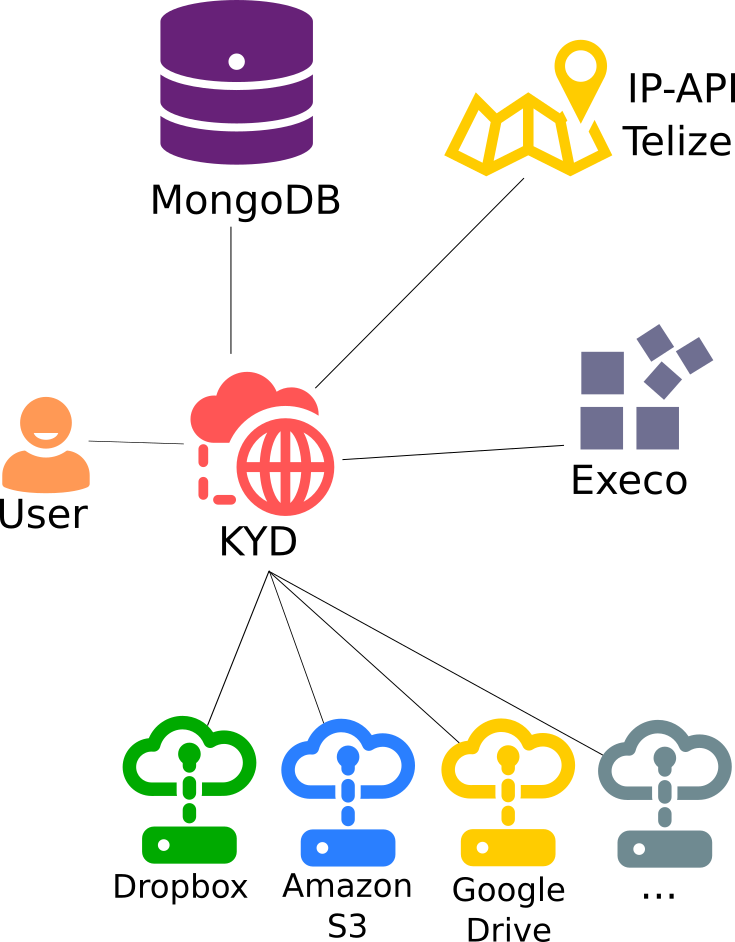
\includegraphics[scale=0.3]{architecture.png}
\caption{Architecture de l'application} \label{fig:archi} \end{figure}

\subsection{Améliorations}

À terme, plusieurs améliorations sont envisageables. Ajouter des paramètres
pour augmenter la précision des tests ferait partie de ces améliorations. Il
serait par exemple possible de vérifier l'efficacité des comptes prémium qui
apportent peut-être de meilleures performances. Il faudrait également compléter
la base de données pour pouvoir répondre le plus souvent possible à
l'utilisateur sans avoir à lui faire effectuer des tests parfois coûteux en
temps. Il serait alors nécessaire d'effectuer des tests à plusieurs
emplacements géographiques dans le monde.

Enfin, une interface Web plus conviviale pourrait rapporter les résultats à
l'utilisateur à la place de la console. Cette amélioration se veut
majoritairement esthétique mais pourrait apporter un certain nombre de
renseignements supplémentaires à l'utilisateur. Notre application n'est pas
encore destinée à des utilisateurs novices (utilisation d'un système
\textit{Unix} et uniquement en terminal), une interface Web pourrait la rendre
plus ergonomique. Enfin il serait intéressant que nos résultats, bien que
stockés dans une base de données, soient plus facile d'accès, en proposant par exemple une liste de résultats pré-établie.


\newpage \section{Analyse des résultats}

Suite à de nombreux tests, nous avons pu obtenir différentes courbes traduisant
les divers aspects de notre projet. Nous désirions comparer les trois
hébergeurs pour une localisation donnée, mais nous voulions aussi savoir s'il
existait des différences selon le moment de la journée ou selon le jour de la
semaine.\\

Pour ces tests, nous avons réalisé un minimum de 15 tests par \textit{Cloud}
et par tranche horaire (par exemple: 15 tests à 15h pour Amazon, GoogleDrive et
Dropbox), les résultats ci-dessous représentent la moyenne de ces tests. Ils
ont tous été réalisés avec les \textit{SDK} de chaque \textit{Cloud}.\\

Pour les figures 1 et 2, les tests ont été réalisés depuis le campus de la Doua
à Lyon 1. Quinze tests ont été effectués en \textit{upload} et en
\textit{download} avec une taille de fichier différente puis la moyenne de ces
tests a permis d'obtenir ces résultats.

\begin{figure}[h] \centering
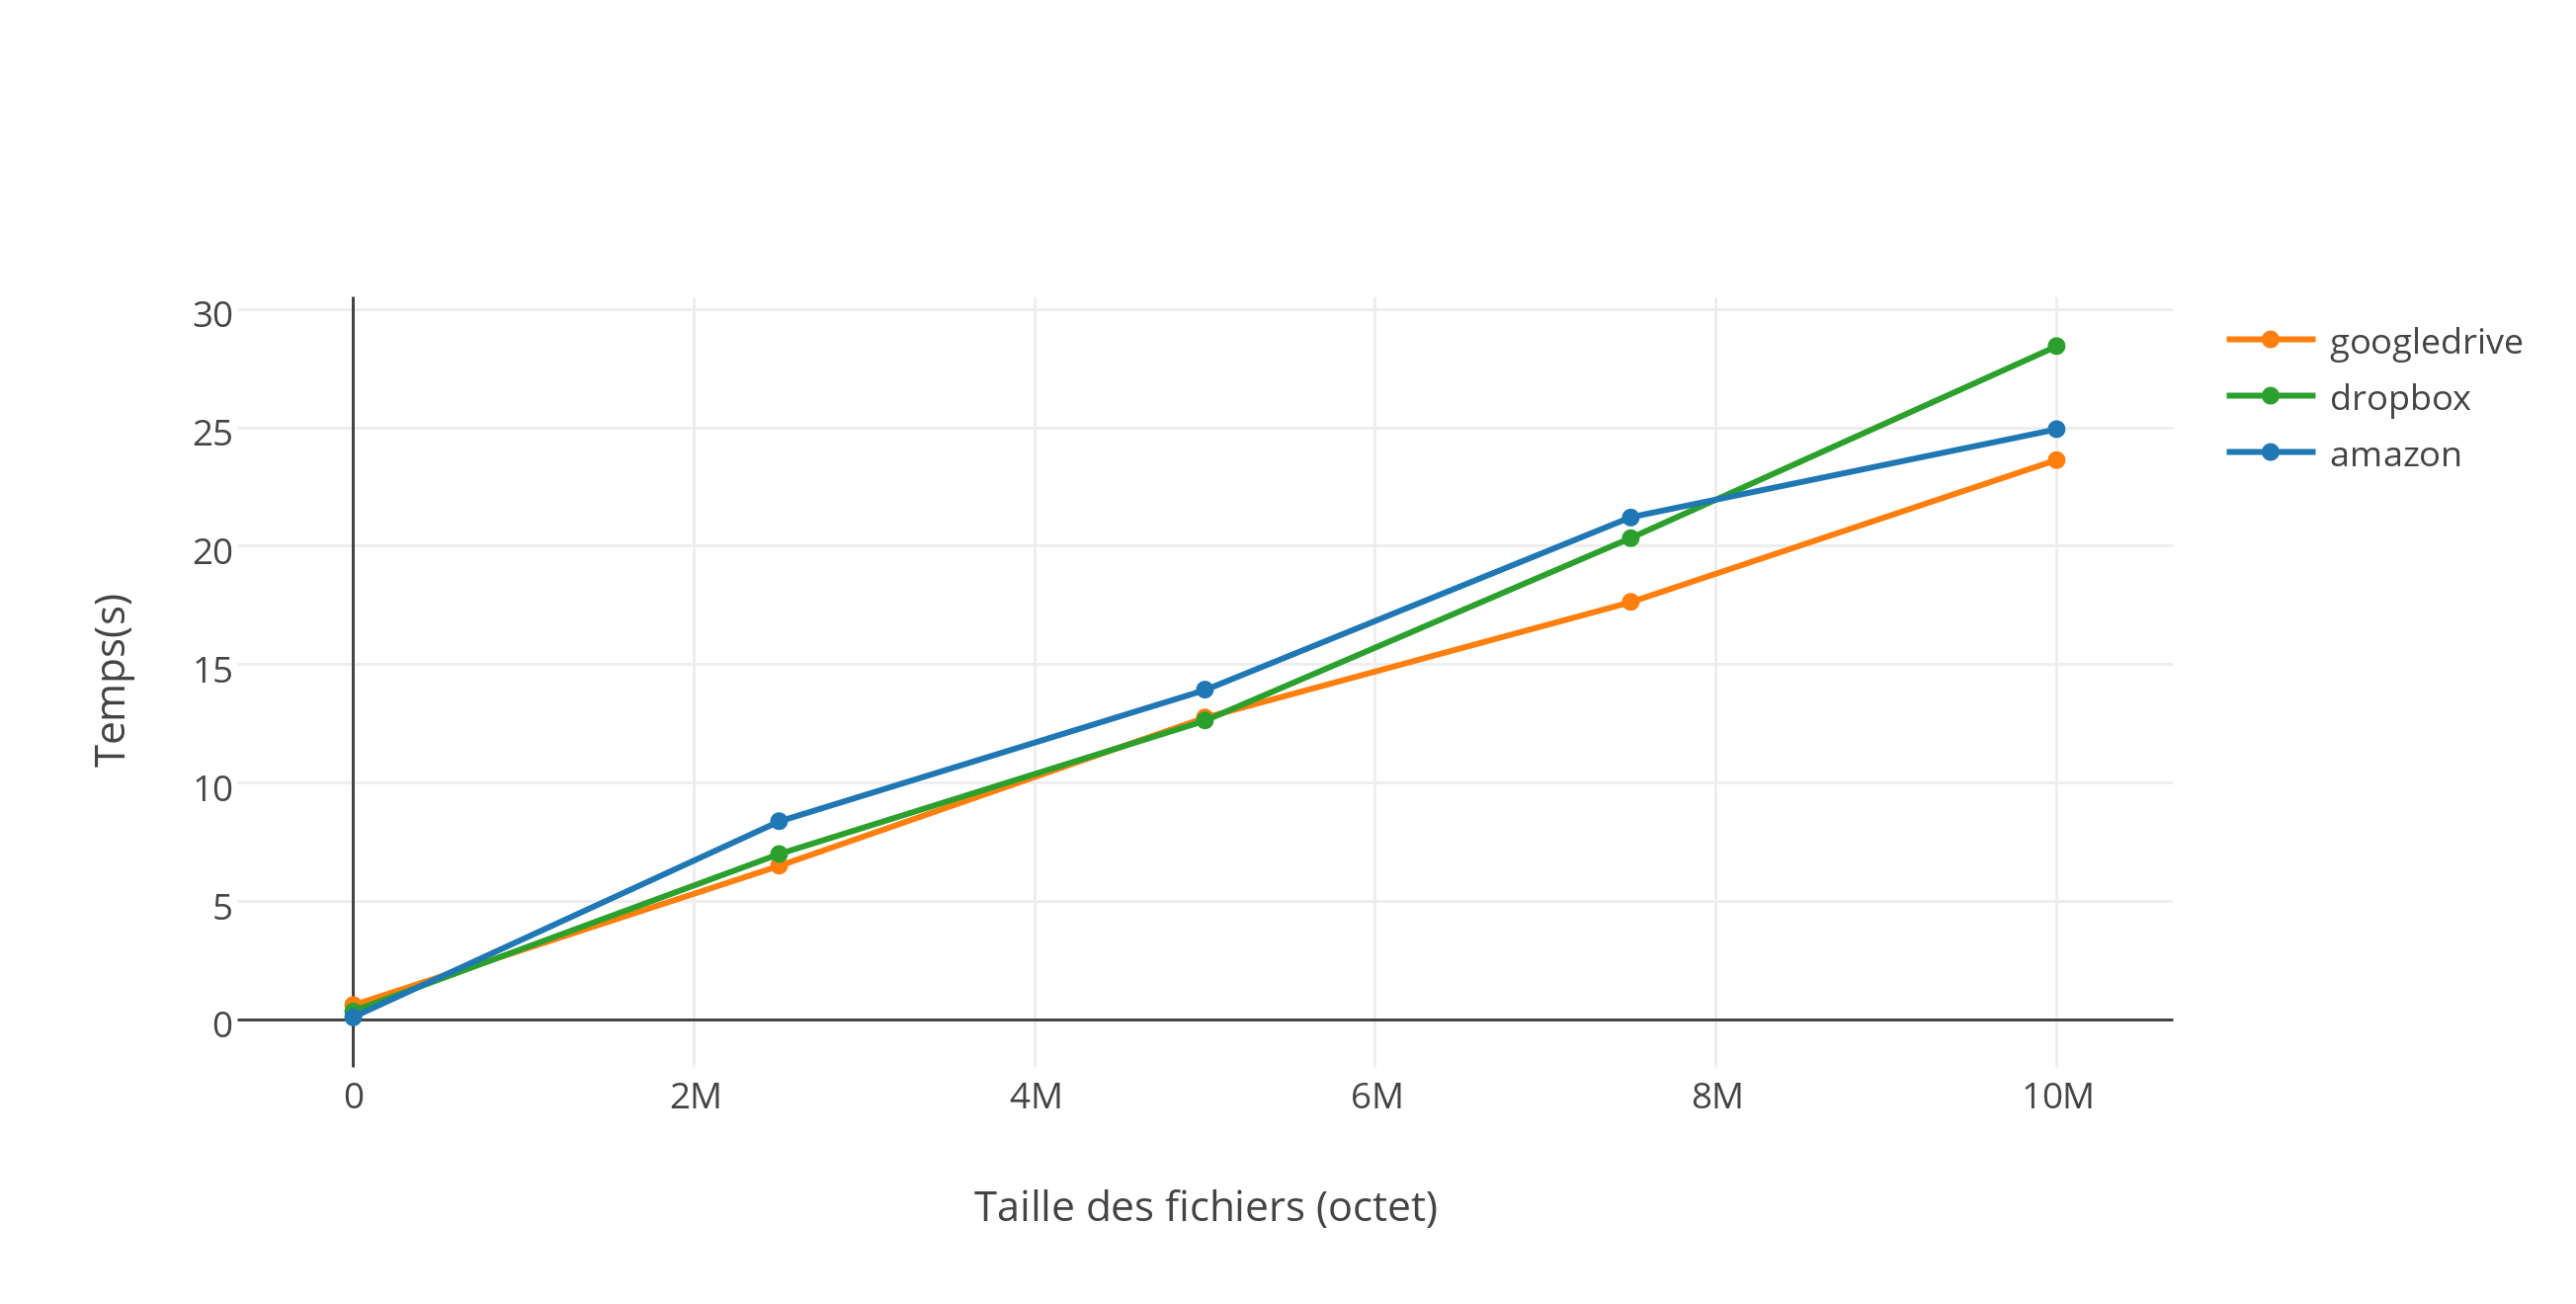
\includegraphics[scale=0.65]{graphe_des_downloads.png} \caption{Graphe des
\textit{downloads}} \end{figure}

\begin{figure}[h] \centering
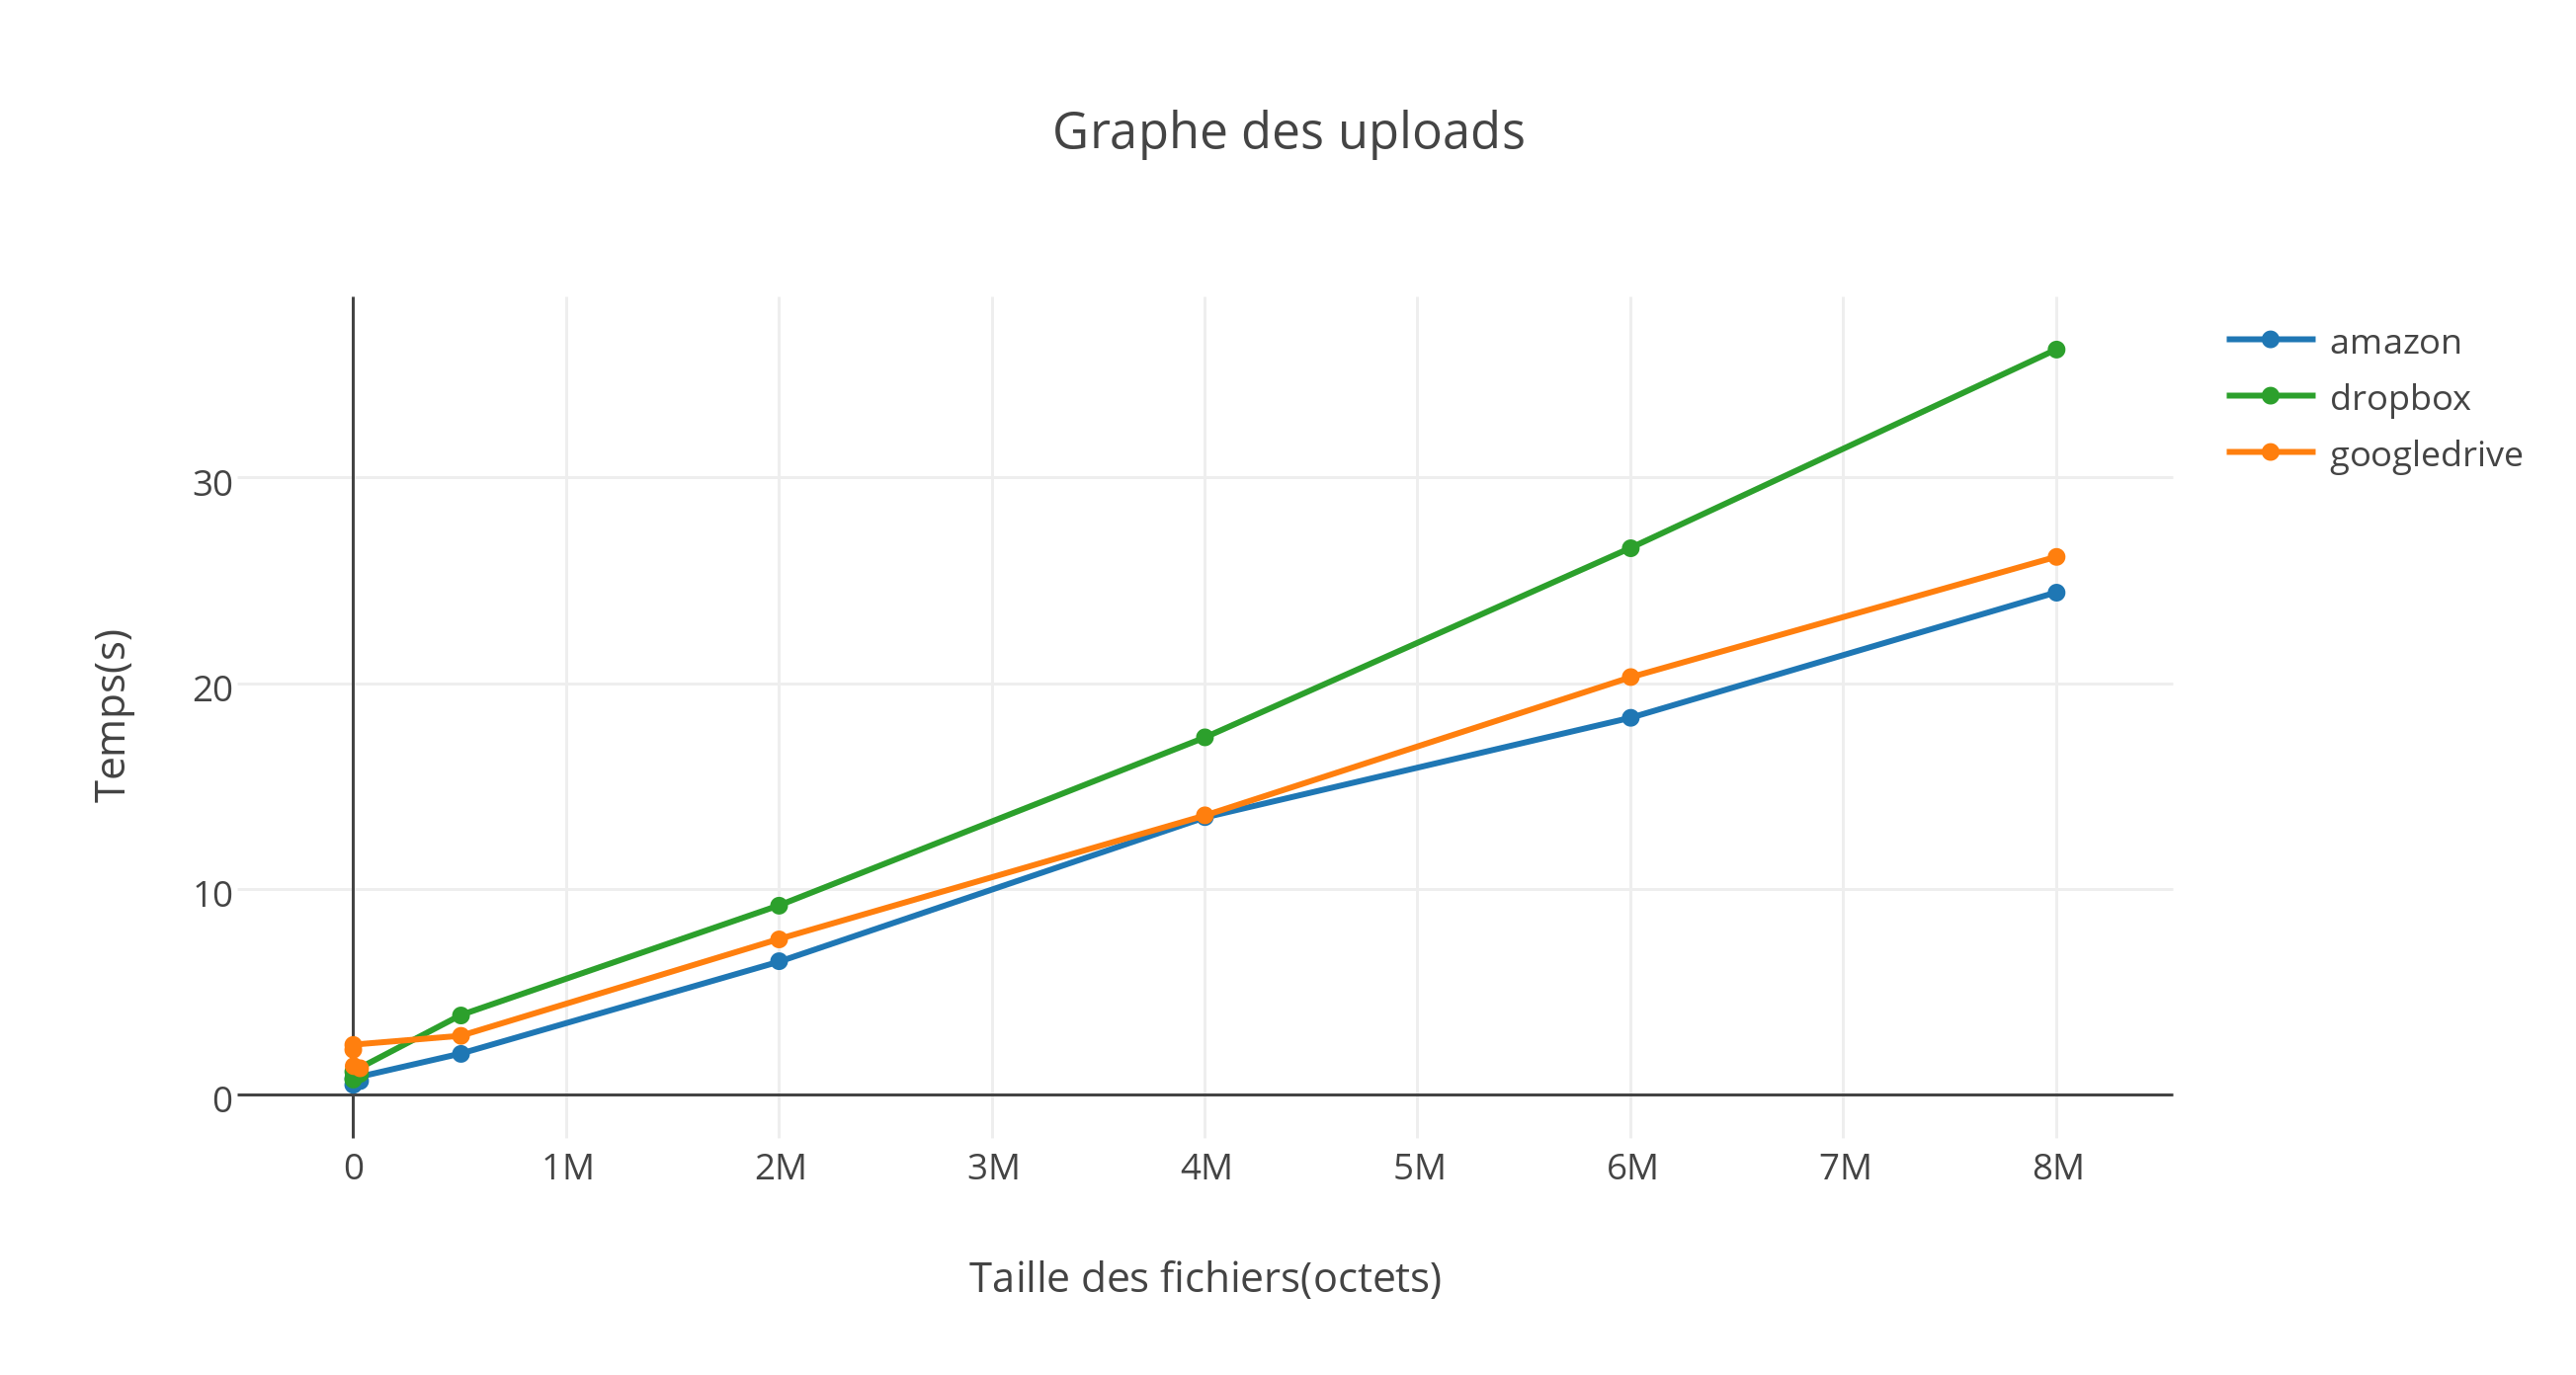
\includegraphics[scale=0.65]{graphe_des_uploads.png} \caption{Graphe des
\textit{uploads}} \end{figure}

On observe une faible différence entre les hébergeurs, seul \textit{Dropbox} semble moins performant mais la différence est assez légère. La différence se creuse plus sur de gros fichiers, mais reste plutôt faible sur le campus de la Doua.\\

Pour les deux figures suivantes, les tests ont été effectués depuis un serveur
virtuel situé à Londres. Ils ont été lancés toutes les heures pendant vingt
quatre heures un dimanche avec une taille de fichier de 10Mo à l'aide de la
crontab du serveur.

\begin{figure}[h] \centering
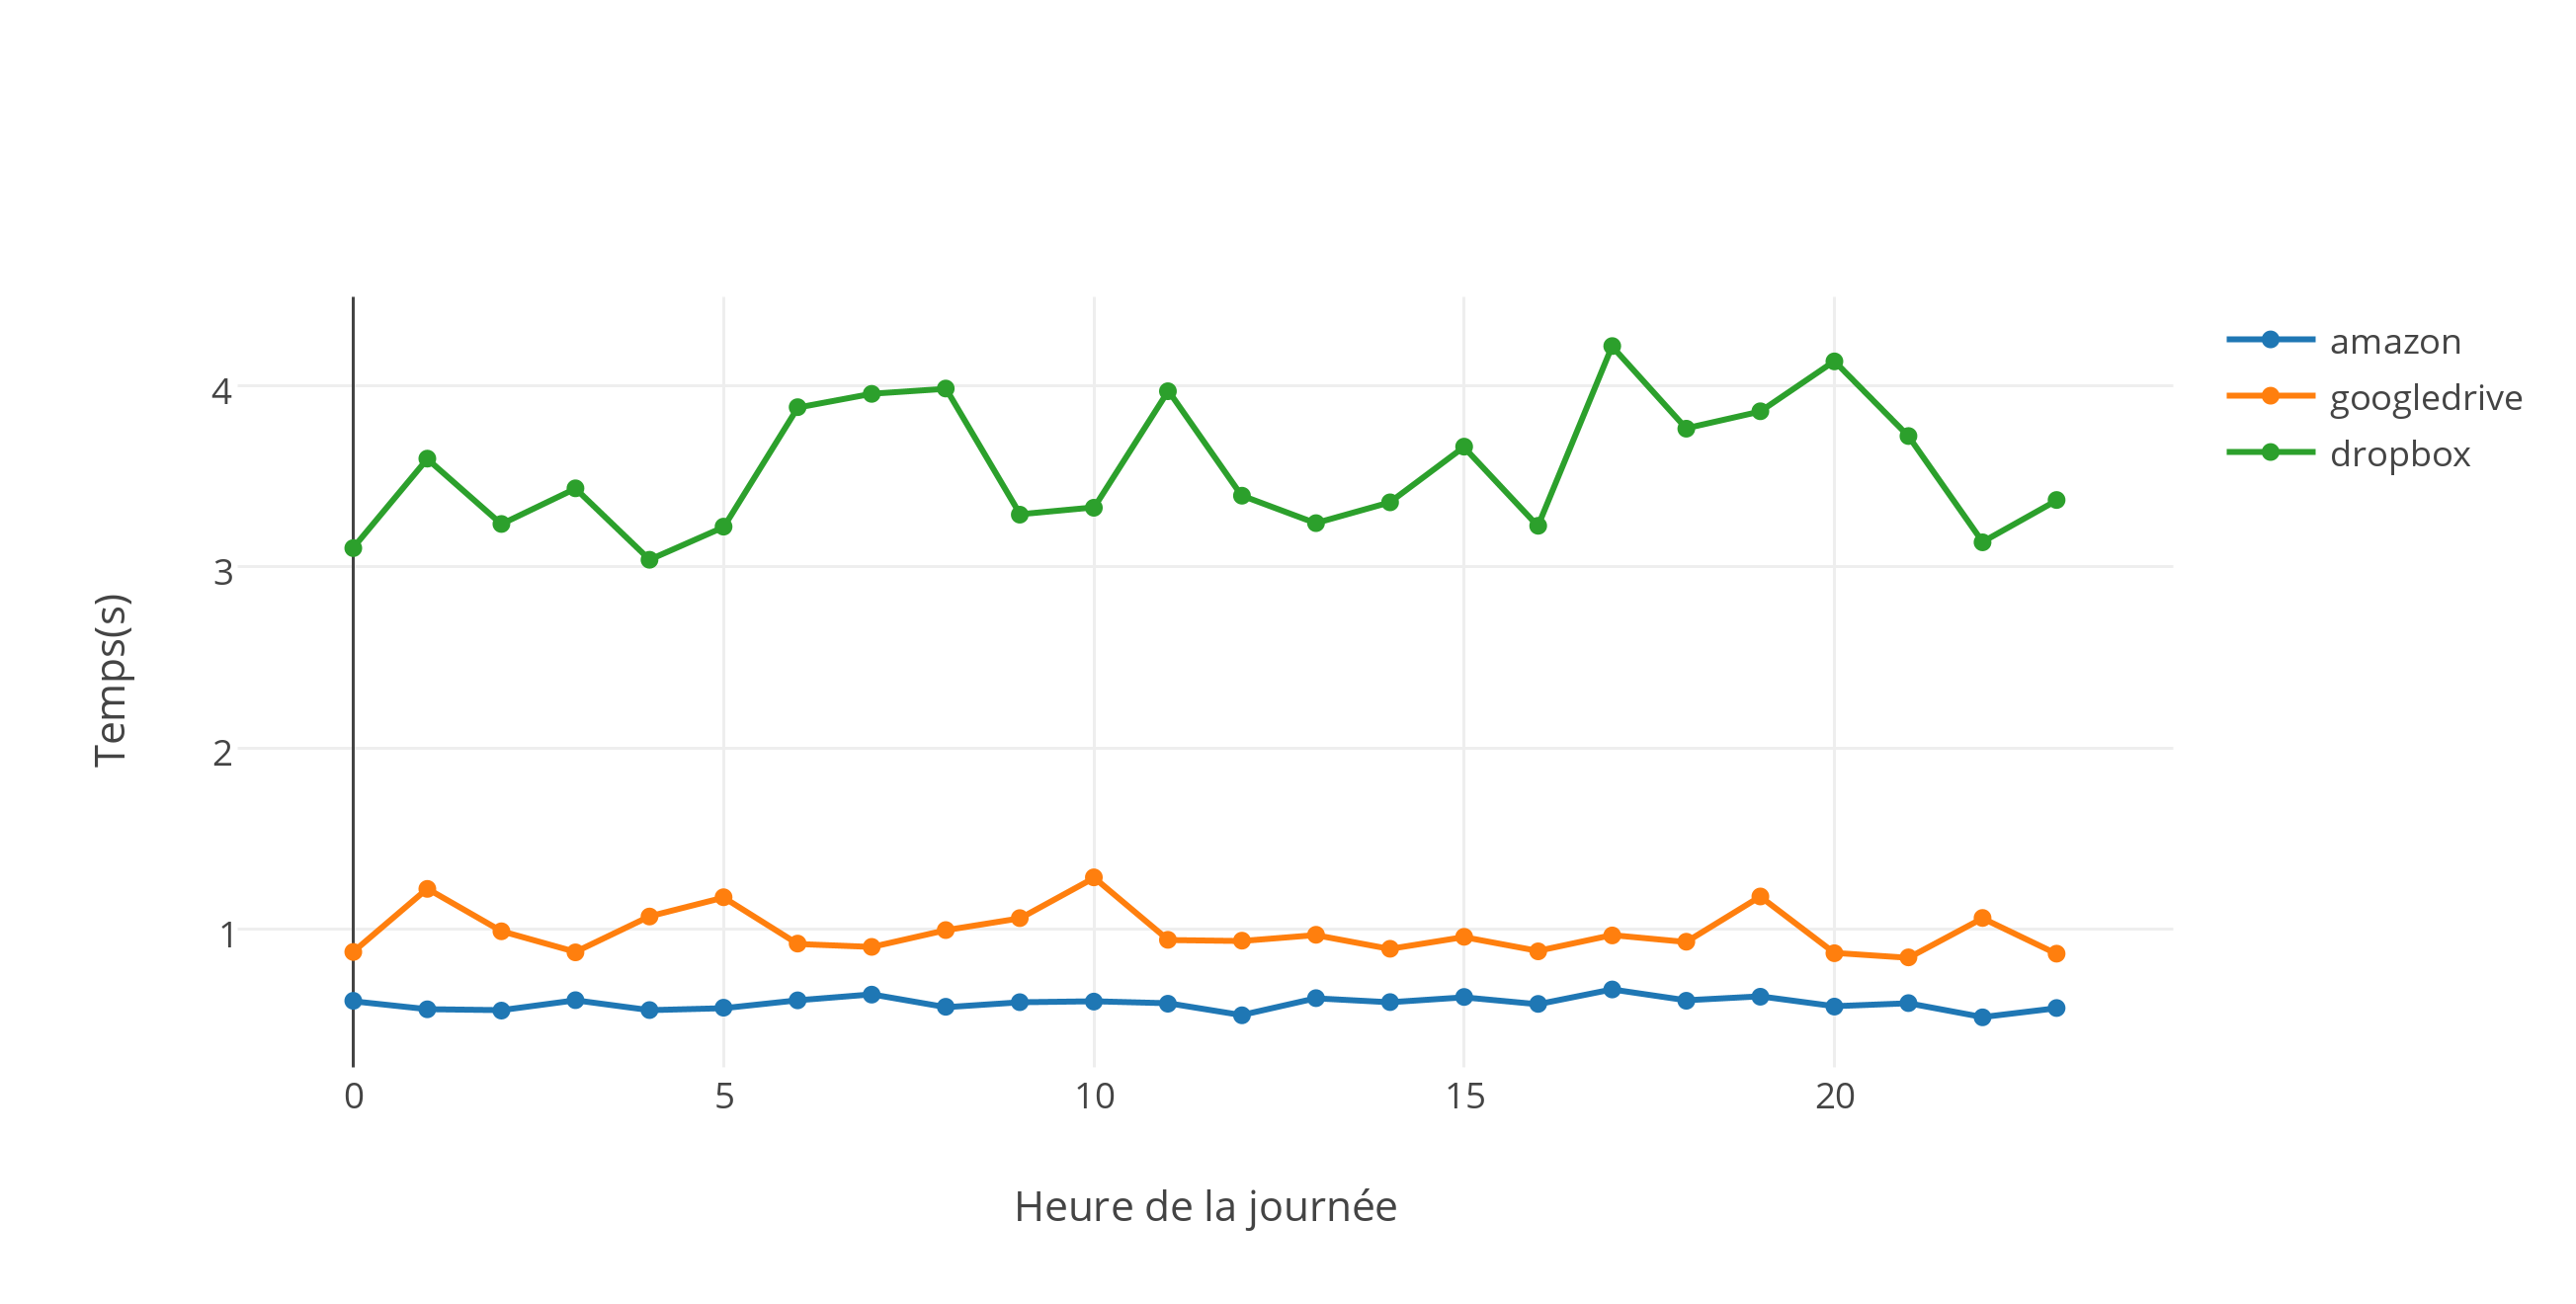
\includegraphics[scale=0.7]{graphe_du_15022015_pour_les_download_de_taille_10mo.png}
\caption{Graphe des \textit{downloads} du 15/02/2015 de taille 10Mo} \end{figure}


\begin{figure}[h] \centering
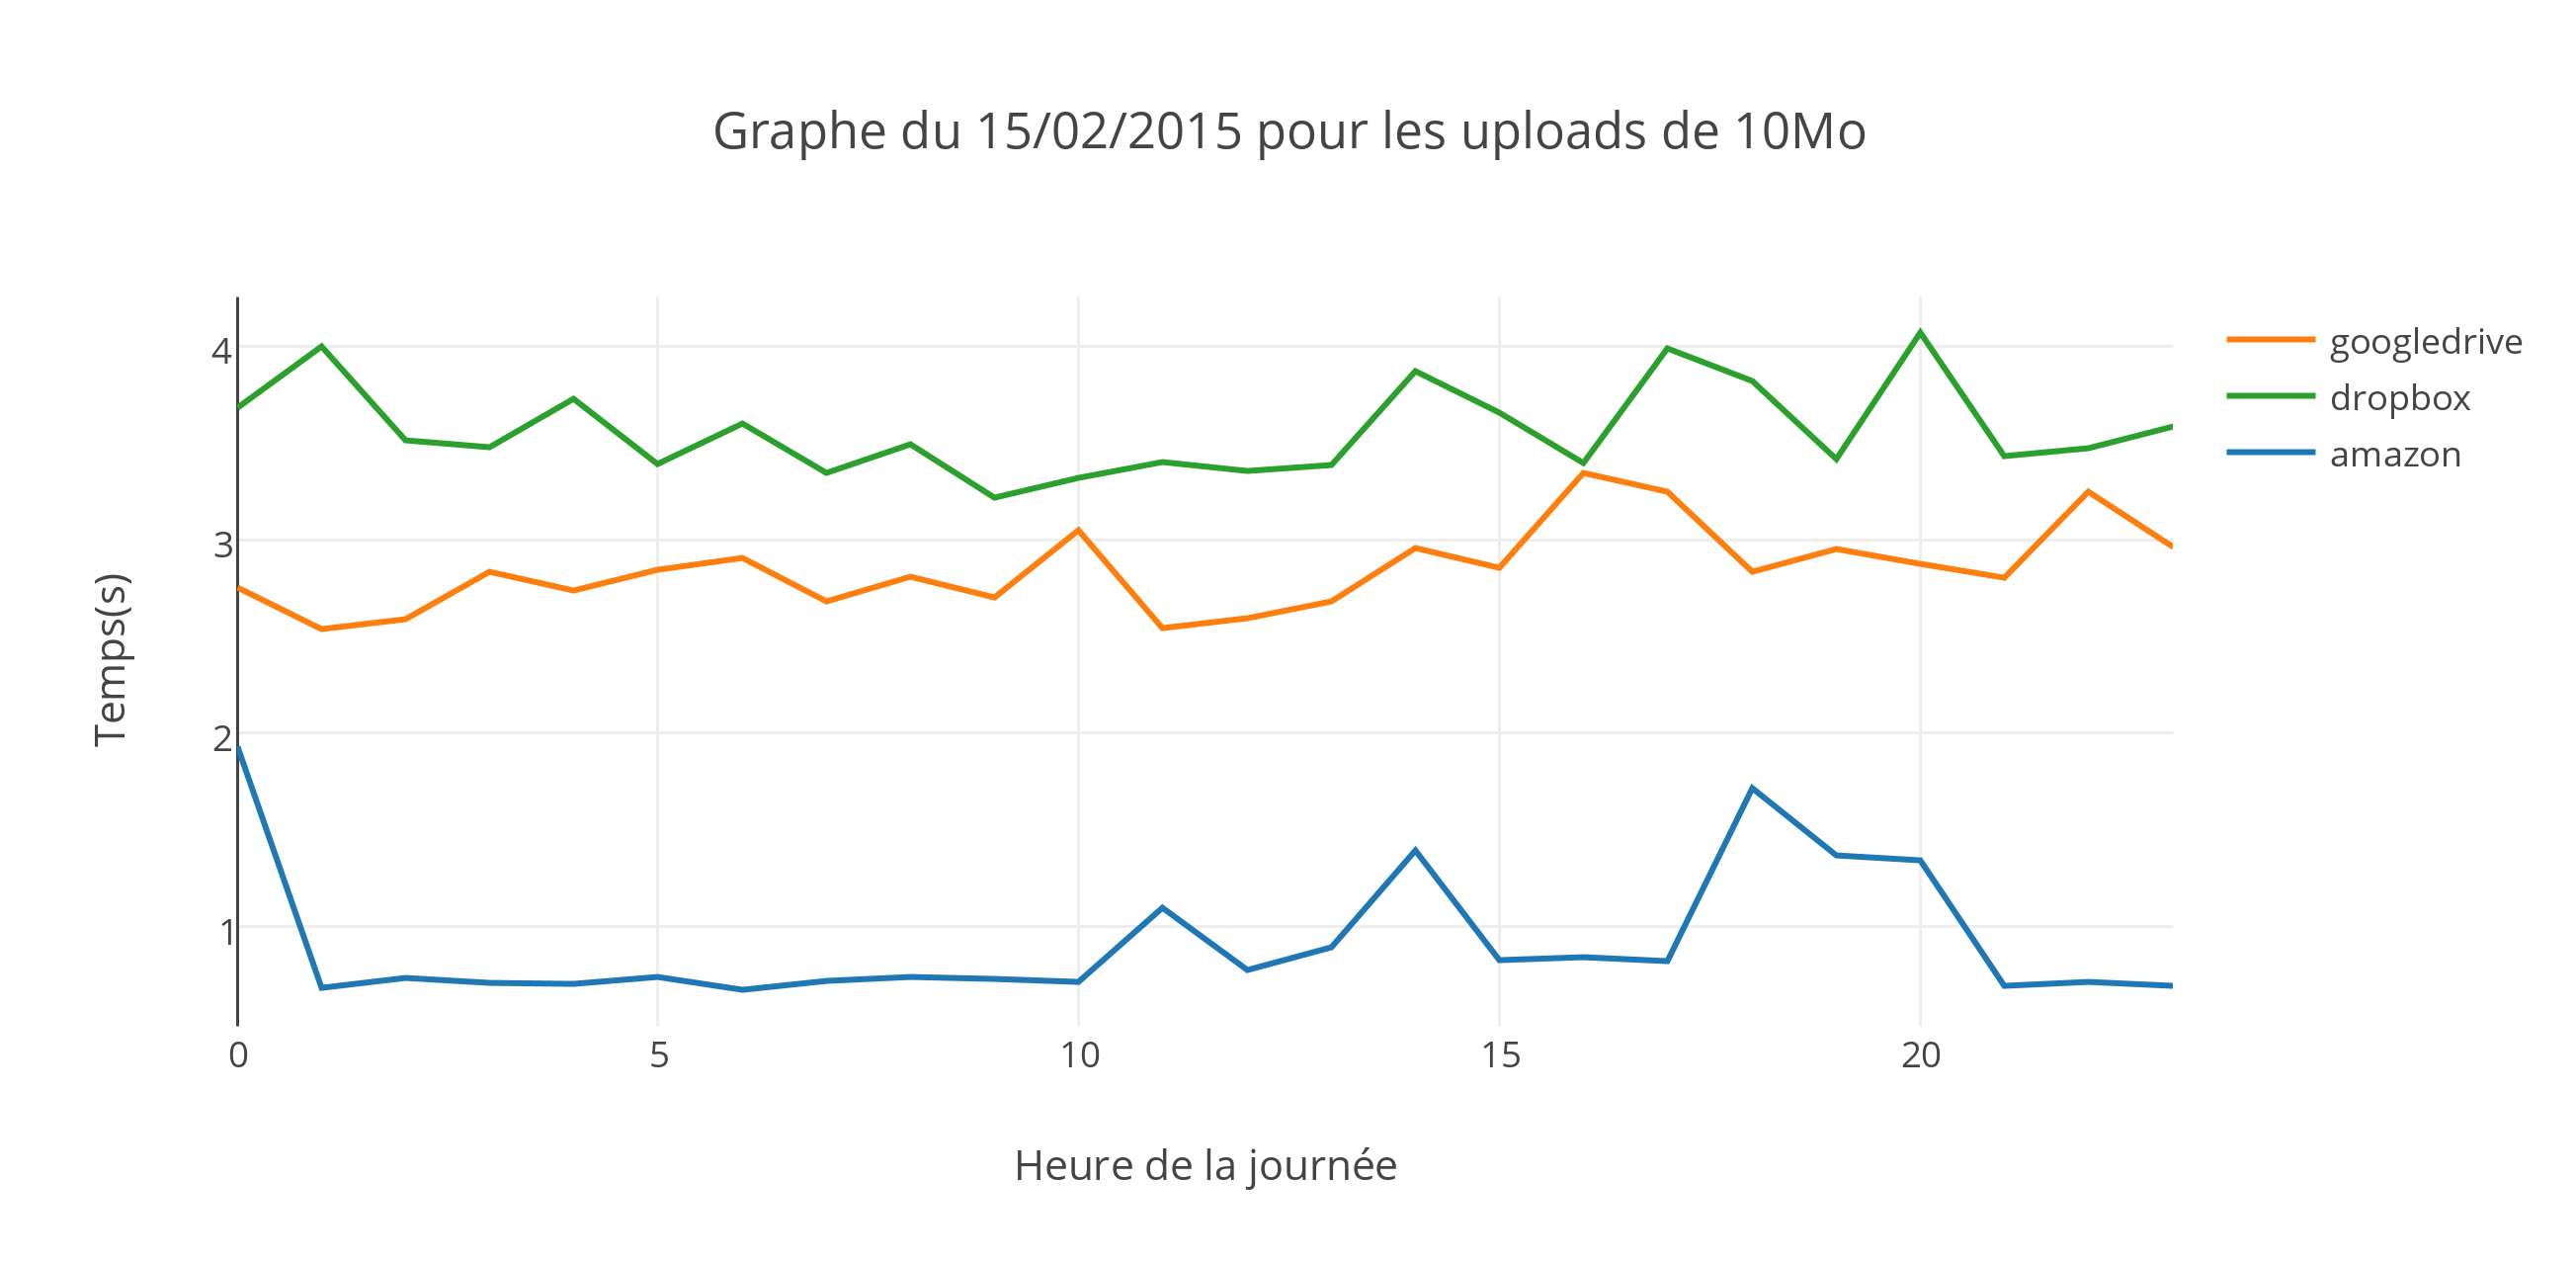
\includegraphics[scale=0.7]{graphe_du_15022015_pour_les_uploads_de_10mo.png}
\caption{Graphe des \textit{uploads} du 15/02/2015 de taille 10Mo} \end{figure}

En \textit{upload}, on observe qu'Amazon suit un schéma connu qui comporte
des pics de latence à 11h, 14h puis entre 18h et 20h. On suppose que cette
situation est due au grand nombre de connexions simultanées durant une plage
horaire plus bondée que les autres. Les performances de Dropbox sont, cette
fois encore, très nettement inférieures à celles de ses concurrents.\\

Dans le même contexte que les deux derniers graphes situés ci-dessus, nous avons
effectué les mêmes tests sur un autre jour de la semaine : le Mercredi.\\

\begin{figure}[h] \centering
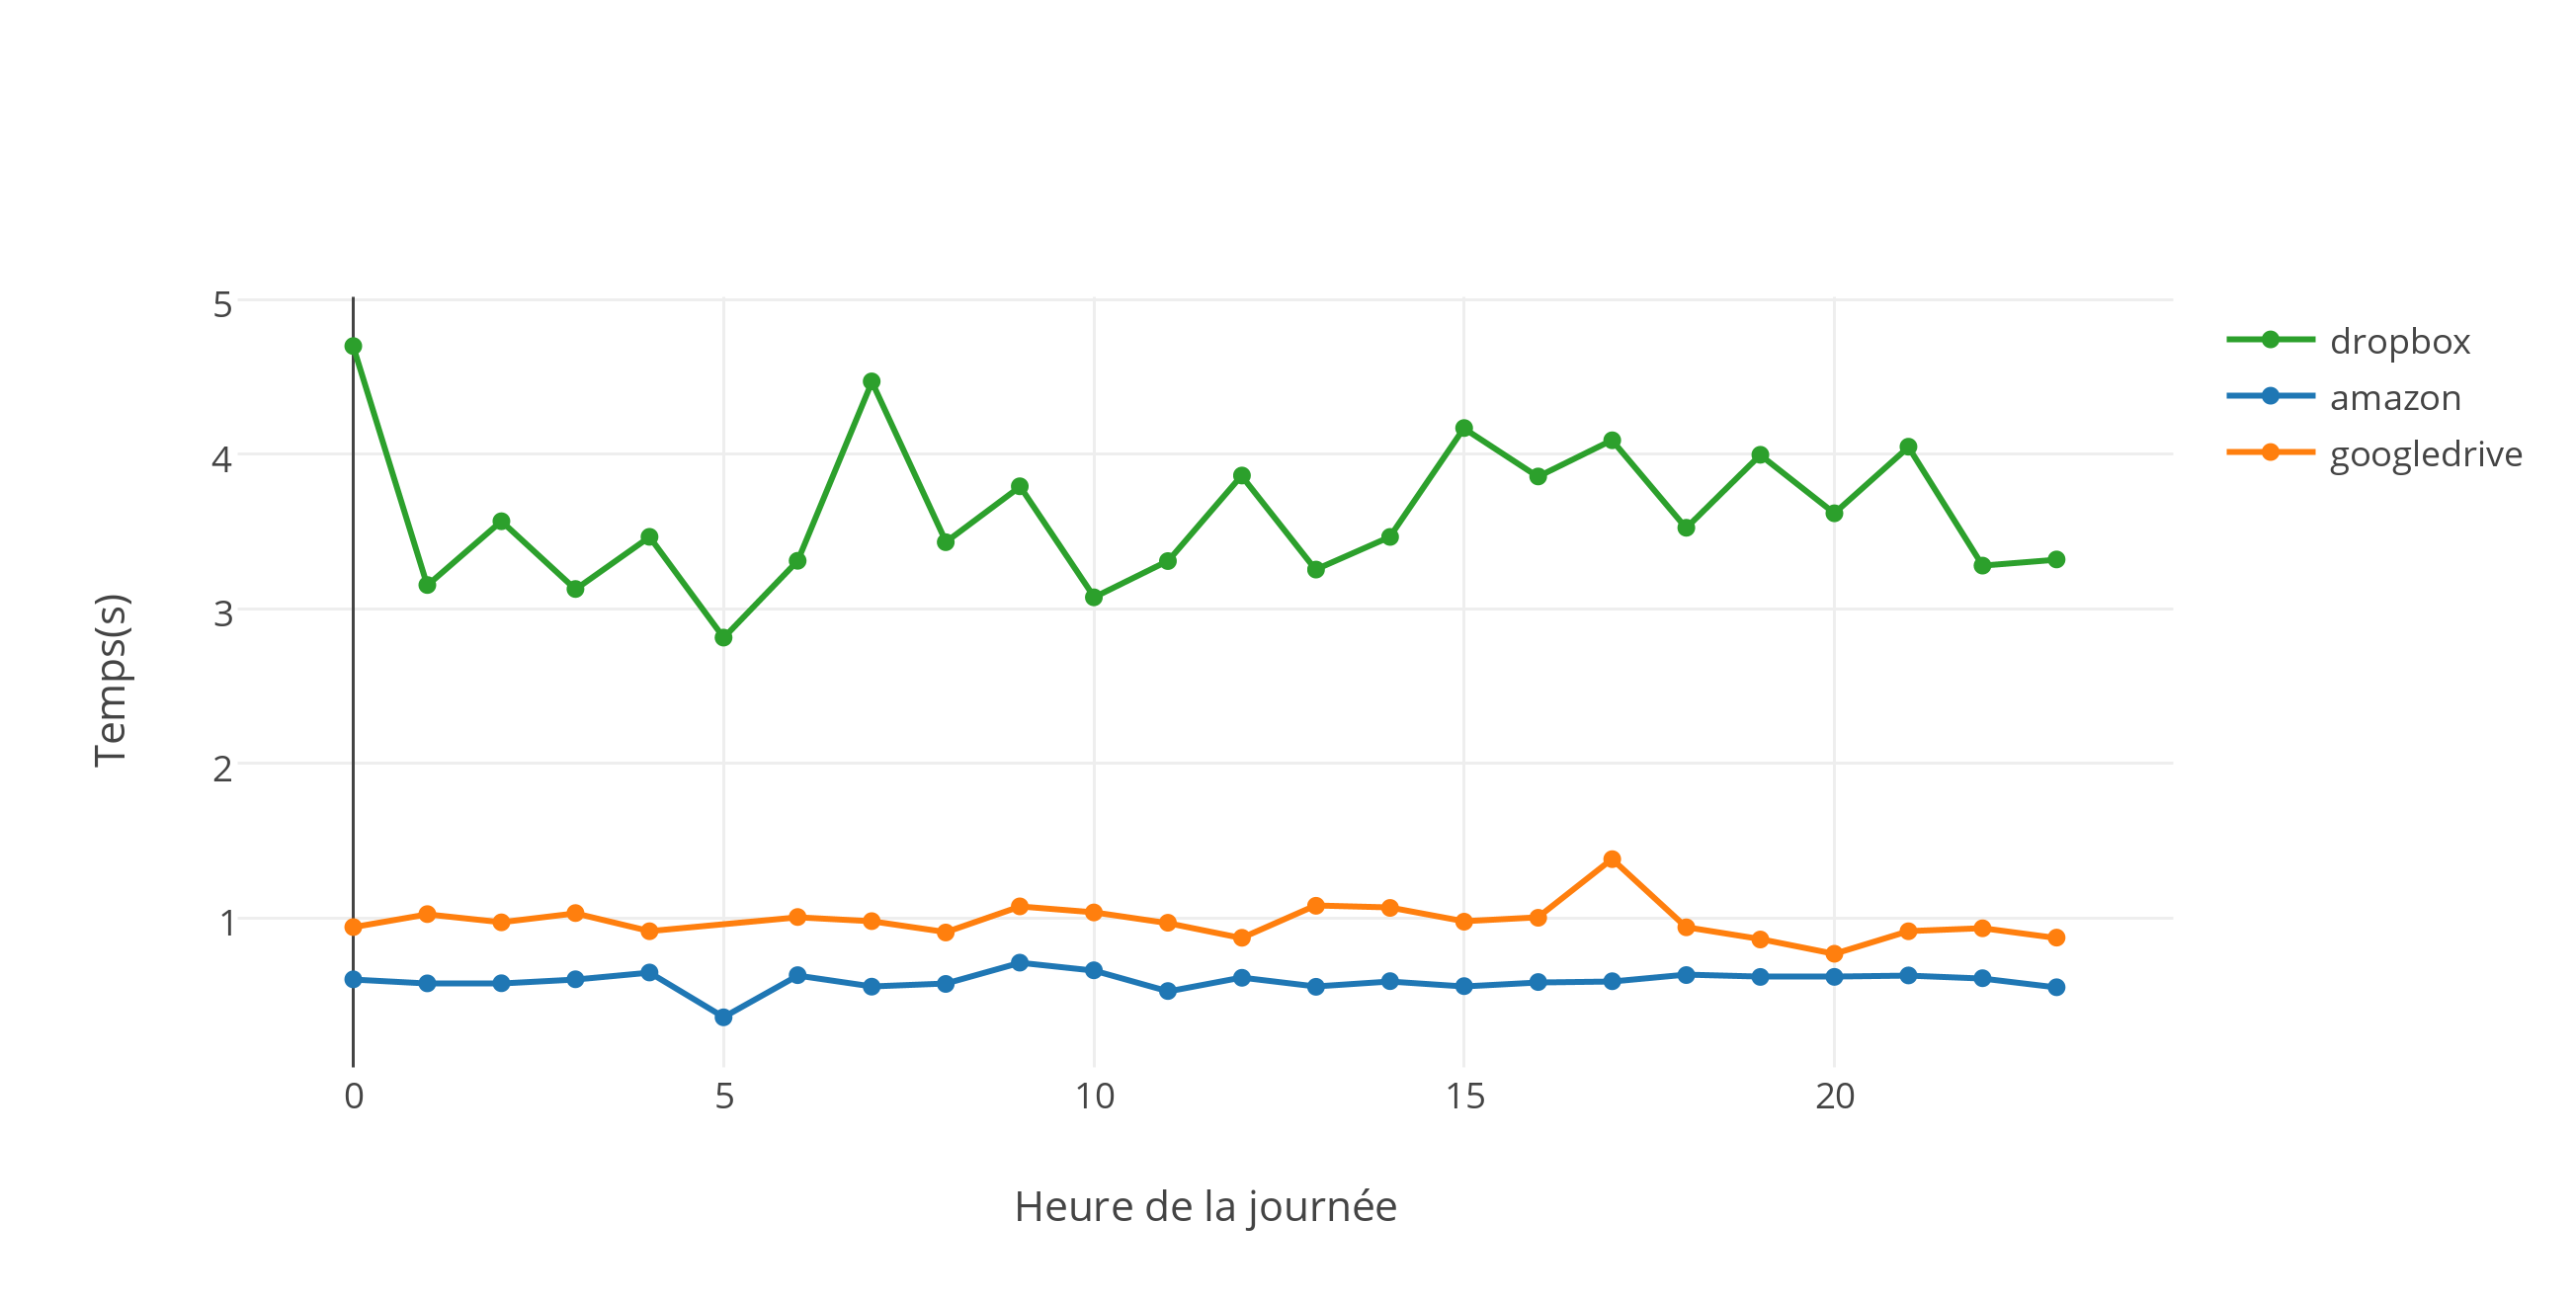
\includegraphics[scale=0.65]{graphe_des_downloads_du_18022015_de_taille_10mo.png}
\caption{Graphe des \textit{downloads} du 15 de taille 10Mo} \end{figure}

\begin{figure}[h] \centering
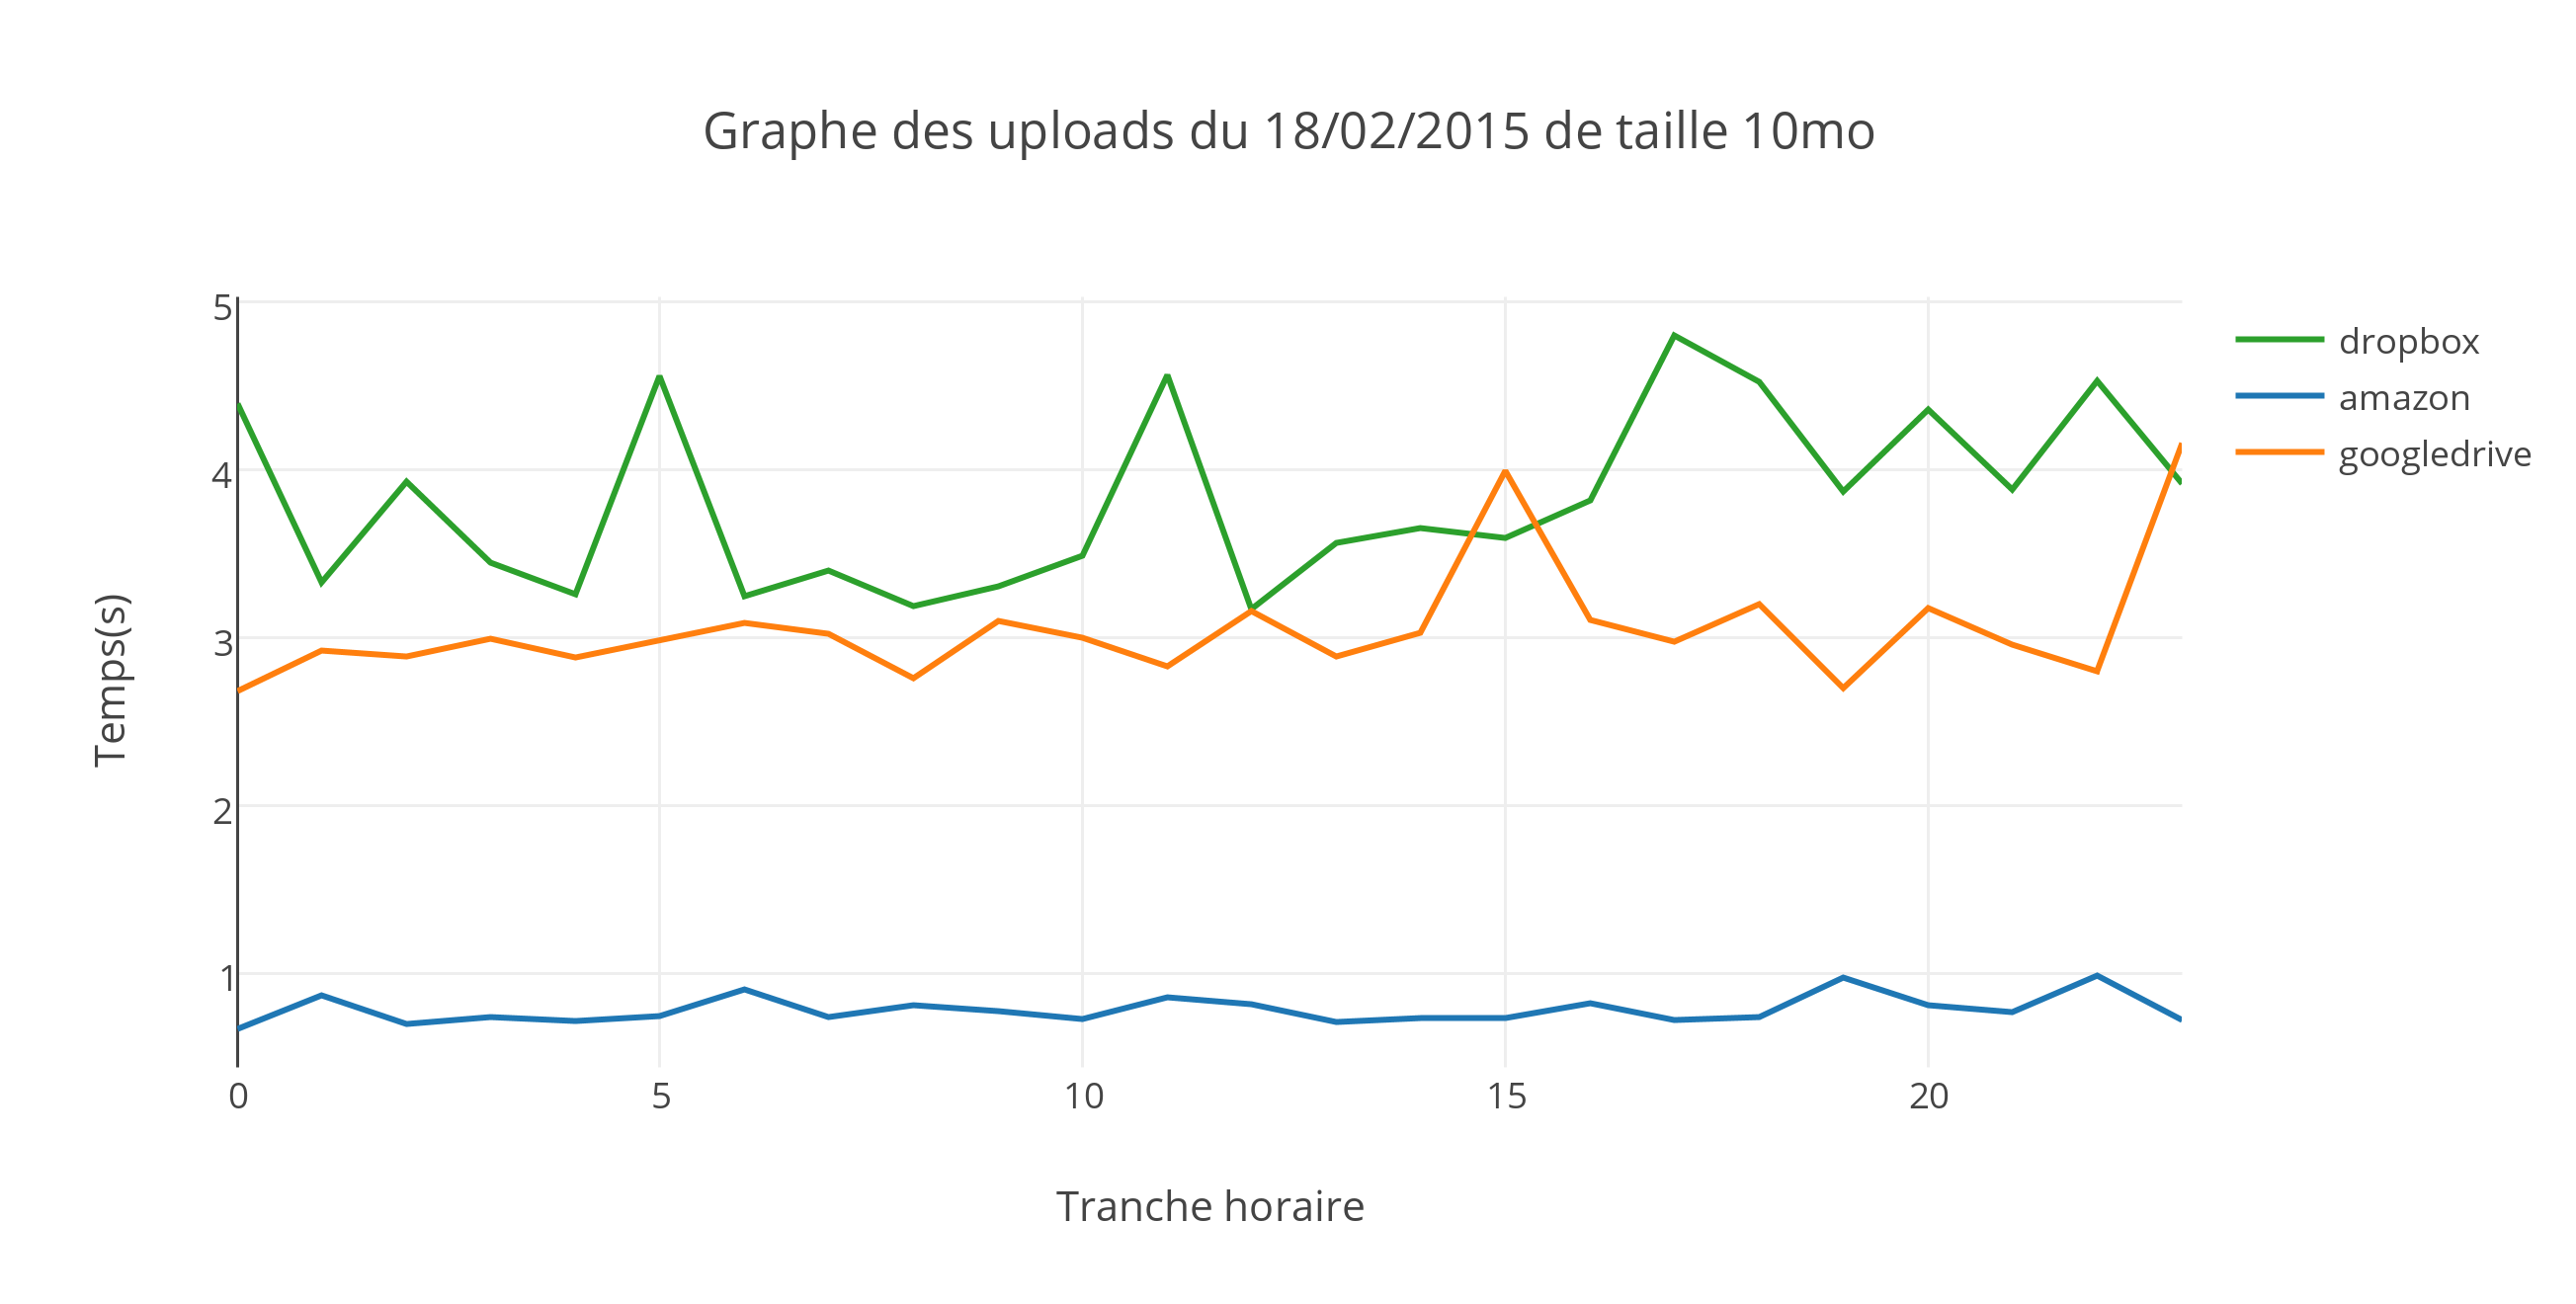
\includegraphics[scale=0.65]{graphe_des_uploads_du_18022015_de_taille_10mo.png}
\caption{Graphe des \textit{uploads} du 15 de taille 10Mo} \end{figure}

On remarque ici l'absence d'une donnée concernant le \textit{Cloud}
GoogleDrive dans la partie \textit{download} car il était en maintenance à 5h
du matin. Notre outil prend en compte ce genre d'erreur et permet de continuer
les mesures sur les autres hébergeurs.\\

On peut observer que l'hébergeur \textit{Amazon} et son service \textit{S3}
reste loin devant les autres \textit{Cloud} en gardant ses moyennes
en-dessous de la seconde.  \textit{Google Drive} possède de bonnes mesures
concernant la partie \textit{download} de son service, cependant on remarque
qu'il rencontre quelques difficultés concernant la partie \textit{upload}.
\textit{Dropbox} reste bon dernier tout au long de ces tests, nous supposons
que cela est probablement due à la surcouche que \textit{Dropbox} ajoute par
rapport à \textit{S3}. En effet, comme nous vous l'avions expliqué plus tôt, le
service \textit{Dropbox} utilise le service d'\textit{Amazon}.\\

La différence entre les résultats de Lyon et ceux de Londres est assez flagrante. Le serveur d'\textit{Amazon} se trouvant en Irlande, on peut supposer que les courbes d'\textit{Amazon} s'expliquent par une plus grande proximité entre le client et le serveur. Les serveurs de \textit{Dropbox} étant partagés avec ceux d'\textit{Amazon}, on aurait pu s'attendre à une courbe similaire. Dropbox n'a donc pas forcément tous ses serveurs aux mêmes emplacements que ceux d'\textit{Amazon} (il n'en possède peut être pas en Irlande).\\

Nous avons calculé l'écart type pour chaque hébergeur pour les quatre derniers diagrammes pour connaître la précision de notre outil. Nous obtenons en moyenne 12\% d'écart avec 16\% pour \textit{Amazon} et 10\% pour les deux autres \textit{Cloud}, ce qui représente un résultat suffisamment précis pour rendre \KYD efficace. Le gros pourcentage d'\textit{Amazon} est fortement augmenté par la courbe des \textit{uploads} du 15/02/2015 qui présente un premier pic inexpliqué (erreurs réseau, difficultés côté serveur ?). Sans ce graphe, \textit{Amazon} propose un écart type de 8\%. Ces résultats sont donc très satisfaisants et prouvent que la précision de notre application correcte.

\section{Conclusion}


Comme dans de nombreux centres de recherche, les chercheurs de l'ENS manipulent de grandes quantités de données parfois très volumineuses. Pour améliorer les performances de ce système, il est nécessaire de minimiser le temps d'accès aux données. Réduire les temps de transfert en choisissant une source de données proche de la destination est une solution envisageable. Il est alors nécessaire de pouvoir sélectionner la meilleure source possible pour migrer ou recopier les données en un minimum de temps.\\

Durant ce projet, nous avons donc analysé, modélisé et implémenté un outil
permettant d'estimer la meilleure solution de transfert de données entre
plusieurs hébergeurs. Pour ce faire, une phase de recherche était nécessaire
puisqu'il fallait vérifier qu'un tel outil n'existait pas déjà et, dans ce cas,
sélectionner les meilleures solutions \textit{Cloud}.\\

Les résultats obtenus suite aux tests ont permis de vérifier la validité de
notre application. En effet, un écart trop important entre les résultats aurait
entraîné un manque d'homogénéité des moyennes. Dans une telle situation,
\KYD n'aurait pas pu fournir de résultat valable puisque les temps 
obtenus auraient été trop aléatoires et nos recherches auraient prouvées qu'un 
tel outil n'était pas réalisable.\\


Ces résultats sont donc très satisfaisants puisque le développement de
\KYD va pouvoir se poursuivre pour proposer des solutions plus précises
sur plus d'hébergeurs. Cette application va très certainement étendre son
champs d'action dans le monde de la recherche puisqu'une poursuite de projet
sera normalement lancée sous peu pour améliorer \KYD.\\

Ce projet est donc une excellente expérience pour nous puisqu'il nous amène sur
un domaine encore très peu exploité et prometteur. Il nous a aussi donné la
chance de pouvoir travailler dans l'univers de la recherche qui nous était
jusqu'alors inconnu et de collaborer avec des chercheurs dans une ambiance
dynamique. Nous avons donc pu faire beaucoup de découvertes au cours de ces
quelques semaines et décider avec plus d'assurance de notre orientation
future.\\

\newpage

\section{Annexes}

Lien du projet sur \cite{Github} : \href(https://github.com/hyptos/kyd){Github/kyd} \\

Notre projet contient environ 2100 lignes de code avec 25 \textit{commit} par semaine en moyenne sur 33 jours.\\

Les outils utilisés :

\begin{itemize}
\item Github - Gestion de version
\item \cite{Travis} - Intégration continue
\item \ipapi et Telize - API de géolocalisation
\item \cite{Execo} - Gestionnaire de processus unix
\item \cite{MongoDB} - Base de données
\item Dépendances python dans le fichier requirements.txt
\item \LaTeX 
\item landscape.io - mesures de qualité du code python
\item Le café du LIP \& du Nautibus
\end{itemize} 

\newpage

\begin{figure}[h] \centering
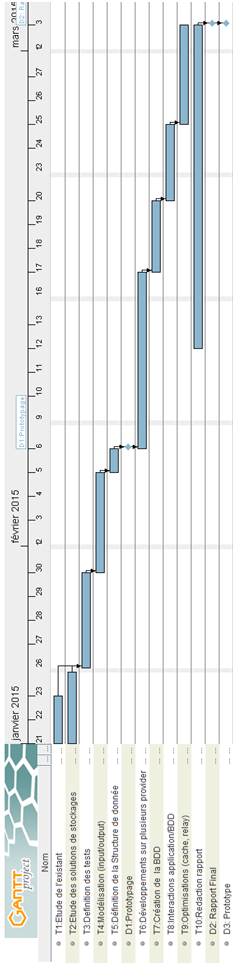
\includegraphics[scale=0.65]{Gantt.png}
\caption{Diagramme de Gantt} \end{figure}
\bibliographystyle{alpha}
\bibliography{biblio}
\end{document}
